\documentclass[12pt,a4paper]{article} 
\usepackage[portuguese]{babel} \usepackage[utf8]{inputenc}
\usepackage{amsmath} 
\usepackage{graphicx}
\usepackage{booktabs}
\usepackage{pgfplots}
\usepackage{tikz}
\usepackage{float}
\pgfplotsset{compat=1.15}
\begin{document}
\setcounter{figure}{1}
\setcounter{section}{2}
\setcounter{page}{6}
\section{Relatório}
\subsection{Introdução}
A resposta em frequência de um sistema linear é uma medida da extensão pela qual senóides de diferentes 
frequências são reproduzidas pelo sistema. Esta resposta em frequência, em um amplificador, é determinado 
pelos capacitores do circuito e as capacitâncias intrínsicas de cada dispositivo.

Deseja-se atuar em uma determinada faixa de frequências em que os efeitos dessas capacitâncias e capacitores sejam desprezíveis, 
o que nos dará um ganho constante. As frequências que estão nesta banda de passagem são chamadas de frequências médias e podem ser vistas entre $\omega_1$ e $\omega_2$ na Figura~2.
\begin{figure}[htpb]
  \centering
  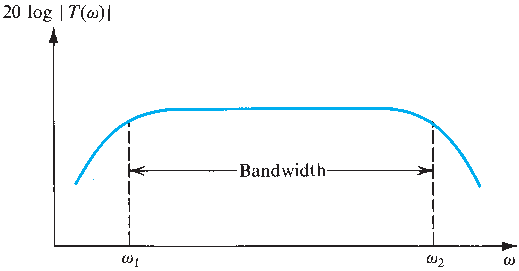
\includegraphics[width=0.8\linewidth]{./img/bandpass.pdf}
  \caption{Diagrama típico para a magnitude de um amplificador, a frequência de corte inferior é indicada por $\omega_1$ e a superior por $\omega_2$.}
  \label{fig:2}
\end{figure}

Esta queda no ganho em baixas frequências estão associadas aos capacitores de bypass e de 
acoplamento, e é interessante pois ganhos em sinais DC é uma característica indesejada para o amplificador.
Já a queda do ganho em altas frequências está associada a capacitâncias parasitas dos componentes.

Utilizaremos nesta prática dois métodos para obter a resposta em frequência do amplificador com transistor bipolar de junção;
reconstrução a partir de amostras e o teste da onda quadrada.

\newpage
\subsection{Análises}

Para o primeiro experimento, montou-se o circuito da Figura~1, um amplificador de emissor comum. 
Aplicou-se um sinal senoidal e verificou-se que a saída não estava distorcida.
Mediu-se o ganho do circuito fazendo um varredura no gerador de sinais em 
toda sua faixa de funcionamento.\\ A partir desta varredura obteram-se os dados dispostos na 
Tabela~1. Desta tabela, pode-se construir o gráfico da magnitude do ganho, em decibéis, pela frequência
em Hertz. Tal gráfico pode ser visualizado na Figura~3.
\begin{table}[htpb]
  \centering
  \caption{Amostras obtidas através da varredura de frequência.}
  \label{tab:label}

  \begin{tabular}{c c}
                   \\ \toprule
    Frequência \emph{(Hz)}  & Ganho \emph{(dB)} \\ \midrule
      1             & 4.46  \\ \midrule
      10            & 7.5   \\ \midrule
      100           & 29.31 \\ \midrule
      1k          & 36.32 \\ \midrule
      10k         & 36.39 \\ \midrule
      100k       & 36.29 \\ \midrule
      1M       & 36.23 \\ \midrule
      5M       & 33.19 \\ \midrule
      10M      & 29.63 \\ \bottomrule
  \end{tabular}
\end{table}
\begin{figure}[htpb]
  \centering
  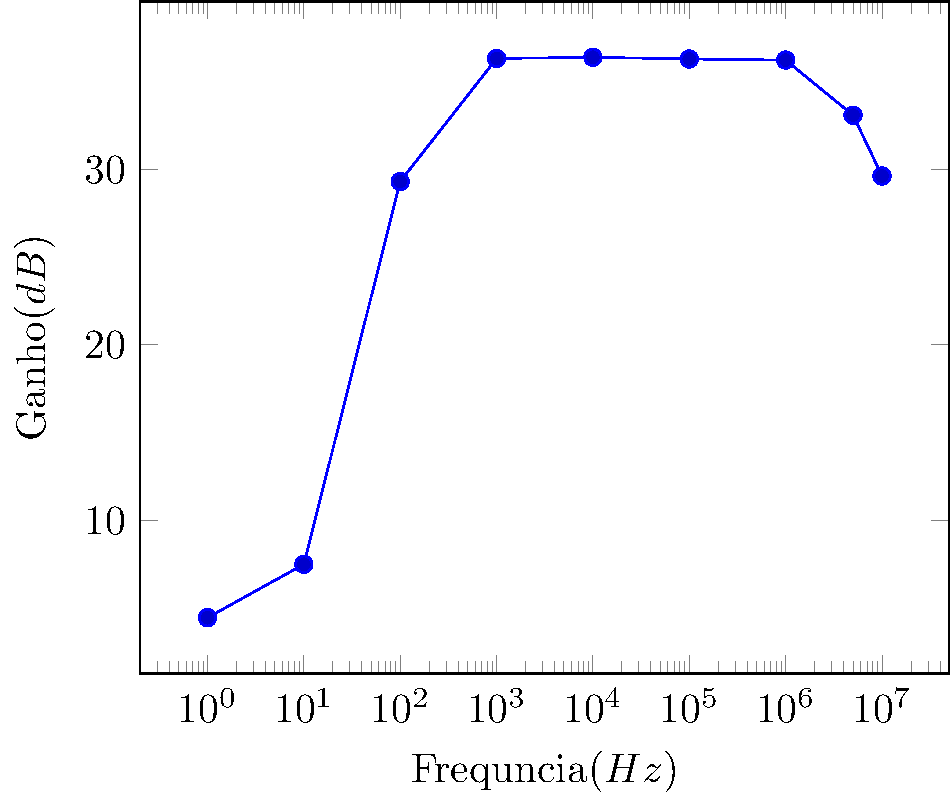
\includegraphics[width=0.8\linewidth]{img/bode.pdf}
  \caption{Resposta em frequência do circuito amplificador emissor comum.}
  \label{fig:3}
\end{figure}

Para o segundo experimento, trocou-se a onda senoidal por uma onda quadrada em que 
a frequência fosse adequada para que pudessemos medir a frequência de corte superior 
e inferior. As Figuras~4-5 indicam as entradas e saídas para uma frequência baixa 
e alta respectivamente que apresentavam os formatos de onda adequados para a estimativa
da frequência de corte inferior e superior. 

Repetiu-se o procedimento anterior trocando o capacitor $C_e$ por um capacitor 
de $4.7\mu F$, obtendo-se as Figuras~6-7.

\begin{figure}[htpb]
  \centering
  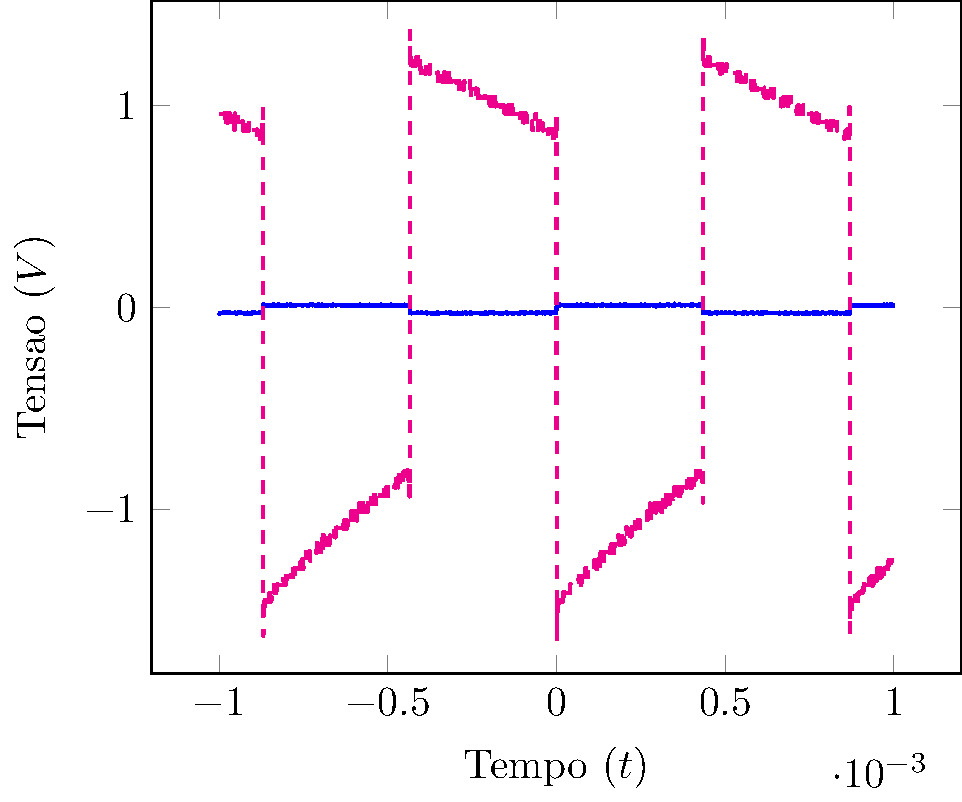
\includegraphics[width=0.8\linewidth]{img/BaixasFreq200u.pdf}
  \caption{Resposta do circuito com capacitor $220\mu F$ para uma onda quadrada (frequência conveniente baixa). Entrada em azul, saída em magenta.}
  \label{fig:4}
\end{figure}
\begin{figure}[htpb]
  \centering
  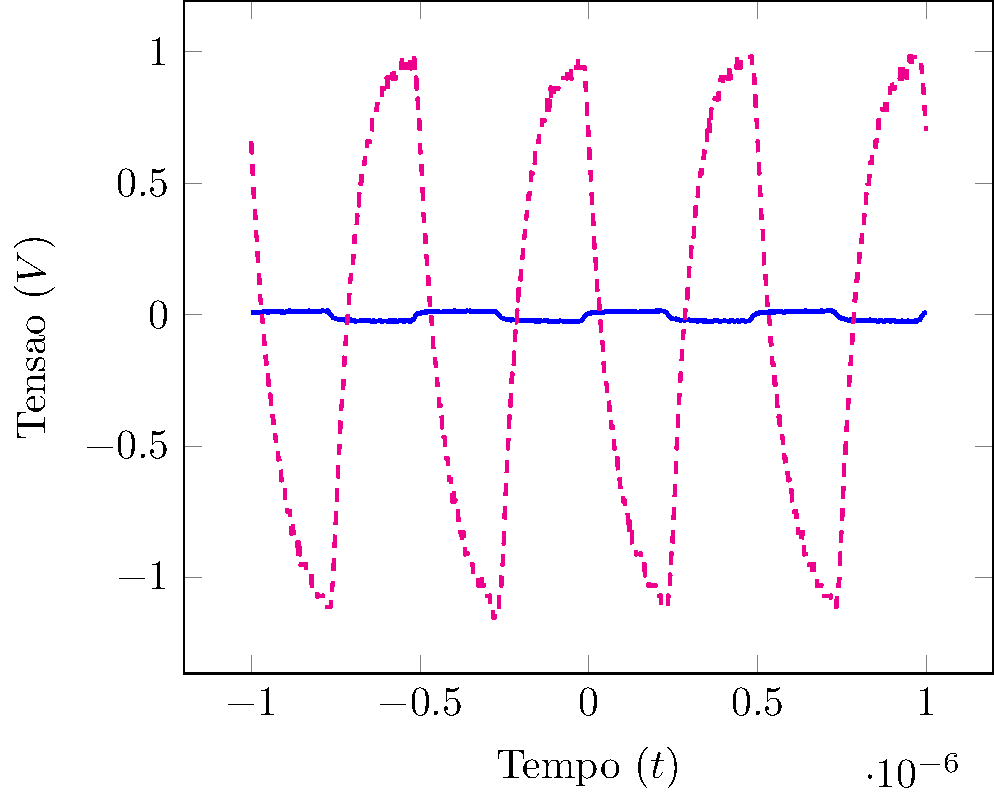
\includegraphics[width=0.8\linewidth]{img/AltasFreq220u.pdf}
  \caption{Resposta do circuito com capacitor $220\mu F$ para uma onda quadrada (frequência conveniente alta). Entrada em azul, saída em magenta.}
  \label{fig:5}
\end{figure}

\begin{figure}[htpb]
  \centering
  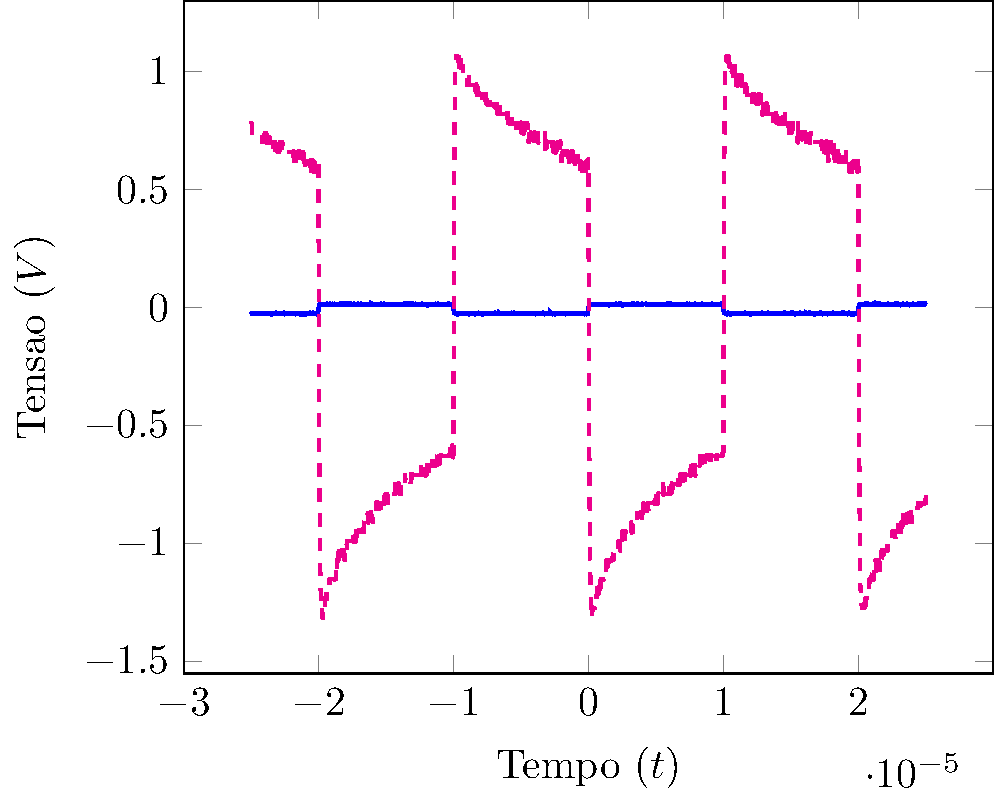
\includegraphics[width=0.8\linewidth]{img/BaixasFreq47u.pdf}
  \caption{Resposta do circuito com capacitor $4.7\mu F$ para uma onda quadrada (frequência conveniente baixa). Entrada em azul, saída em magenta.}
  \label{fig:6}
\end{figure}
\begin{figure}[htpb]
  \centering
  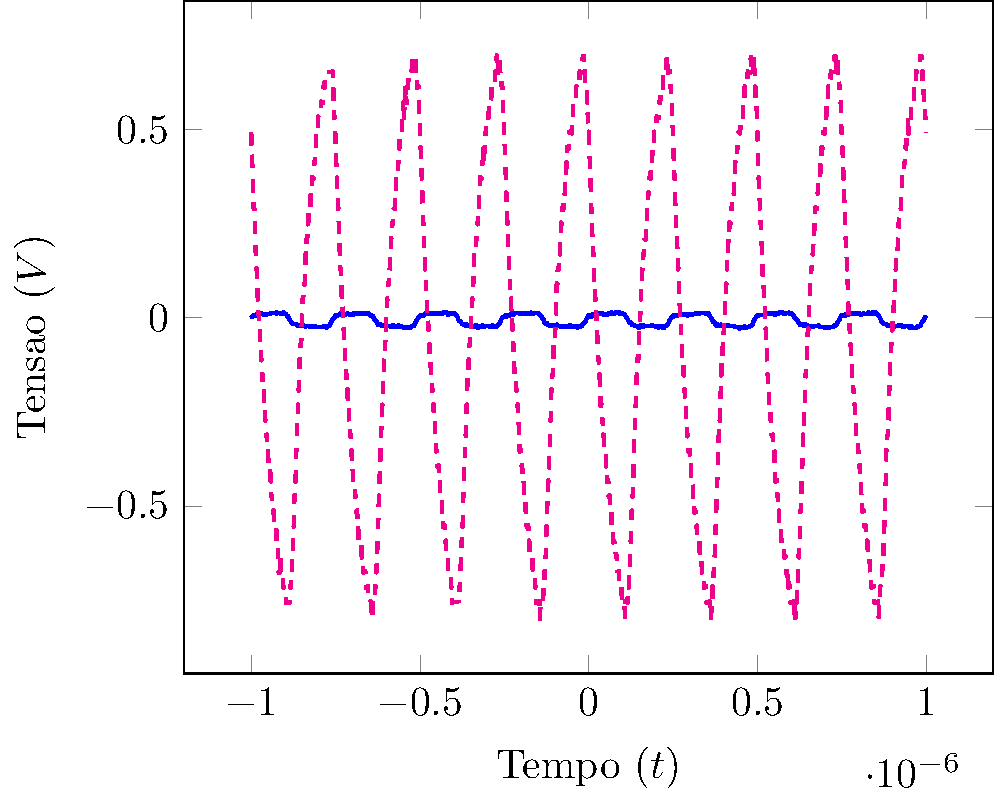
\includegraphics[width=0.8\linewidth]{img/AltasFreq47u.pdf}
  \caption{Resposta do circuito com capacitor $4.7\mu F$ para uma onda quadrada (frequência conveniente alta). Entrada em azul, saída em magenta.}
  \label{fig:7}
\end{figure}
\newpage

\subsection{Discussões}
Podemos então analisar a Figura~2 que foi gerada a partir da Tabela~1 referente ao experimento 1.
Nela podemos encontrar valores 3dB abaixo do ganho fornecido pelo circuito na banda de passagem 
em frequências acima e abaixo desta banda. Definiu-se então através deste gráfico, construído a partir de
interpolação de dados amostrados, as seguintes frequências de corte:
\begin{align}
  f_{ci} = 425 \text{Hz} \\
  f_{cs} = 5 \text{MHz}
\end{align}

No segundo experimento medimos a incilinação na saída para 
uma entrada com aplitude e com frequência convenientes. 
Calculou-se então o valor teórico, segundo o método da onda quadrada,
para a frequência de corte inferior:
\begin{align}
  D= \frac{V_1- V_2}{V_1}  = \frac{1240.25mV - 840.51mV}{1240.25mV} = 0.323 \\
  f_{ci}= \frac{D \times f_{Q}}{\pi}= \frac{0.323 \times 2.03 \text{kHz}}{\pi}=208 \text{Hz}
\end{align}

Para encontar o valor da frequência de corte superior, mediu-se  em uma frequência 
conveniente, o tempo de subida necessário para que o valor vá de 10 a 90\% 
do valor final. Assim, calculamos a frequência de corte superior teórica:
\begin{align}
  t_{r} = T_2 - T_1 = 511ns - 407ns =104ns\\
  f_{cs}= \frac{0.35}{t_r}= 3.36 \text{MHz}
\end{align}

Percebe-se aqui que apesar dos resultados teóricos (método da onda quadrada) e 
experimentais (método da varredura) apresentarem resultados de mesma ordem de grandeza,
ambos resultados estão de certa forma distantes. Podemos alegar que isto se deve 
a imprecisão de ambos os métodos que são apenas aproximações e que este erro 
foi agravado pela falta de um maior conjunto de dados no método experimental, dado 
que quanto mais dados amostrados, mais fidedigno é o resultado.

Em seguida, repetiu-se o método da onda quadrada para o mesmo circuito da Figura~1,
apenas com o capacitor $C_{e}$ trocado por um de $4.7\mu F$. Desta forma repetimos 
o equacionamento acima:
\begin{align}
  D= \frac{V_1- V_2}{V_1}  = \frac{1060 mV- 578mV }{1060 mV} = 0.455 \\
  f_{ci}= \frac{D \times f_{Q}}{\pi}= \frac{0.455 \times 101 \text{kHz}}{\pi}=45.955\text{kHz}
\end{align}
\begin{align}
  t_{r} = T_2 - T_1 = 756ns- 632ns=124ns \\
  f_{cs}= \frac{0.35}{t_r}= 2.82 \text{MHz}
\end{align}

Desta forma, podemos perceber que a banda de passagem do circuito tem dependência 
direta com o valor de $C_e$. Presume-se que quanto menor for o valor de $C_{e}$, 
menor a banda de passagem de um circuito amplificador.
\newpage
\subsection{Conclusão}
Nesta prática estudou-se a resposta em frequência em amplificadores constituídos 
de transistores bipolares de junção na configuração emissor comum. 

Para estimarmos as frequências de corte superior e inferior, utilizou-se dois métodos, 
o método da varredura e o método da onda quadrada. Ao utilizarmos o método da varredura,
amostramos diversos ganhos em frequências diferentes e traçamos um um gráfico 
em que pode-se estimar as frequências de corte superior e inferior. 

No método da onda quadrada, encontramos frequências que eram convenientes para que 
a saída da onda estivesse adequada para aplicar o método e aplicamos equações que 
teorizavam os valores da frequência de corte inferior e frequência de corte superior. 

Percebeu-se então que os valores de ambos métodos diferiam razoavelmente. Supomos que 
esta diferença se dava pela não exatidão de ambos os métodos e que esta fora agravada 
pela falta de um conjunto de dados maior no método da varredura. 

Ao aplicarmos o método da onda quadrada para um capacitor diferente, também pode-se perceber
que a valor da capacitância de bypass, $C_{e}$, é relacionada a largura da banda de passagem 
do circuito, e que quando menor este valor, mais estreita será esta banda, concluindo assim
nosso estudo sobre respostas em frequências.
\end{document}
